\graphicspath{{../06Applications/pics/}}

\chapter{Applications}\label{ch:Applications}
\lettrine[lines=2]{\color{darkocre}W}{e} are now ready to appreciate
how tensors are used in ``real life''. In this chapter we will
encounter examples of
tensors that are used in mathematics, physics, and engineering. 

\begin{myprereq}{Prerequisite Knowledge}
	To fully understand the material of this chapter, readers should be comfortable with the following concepts:
	
	\begin{itemize}
		\item \phantom{phantom}
		\vspace{-0.5cm}
		\item State
		\item Dynamical equations
	\end{itemize}	
\end{myprereq}

\section{Hydrogen-like Atoms}
We will start with the simplest atomic system: Hydrogen atom.

\subsection{Hydrogen Atom}
The most abundant element in the observable universe is hydrogen. A
hydrogen atom has two components: heavy nucleus (proton) and light
``shell'' (electron). The two components can be separated in the
process of \emph{ionization}. A significant energy is required to
tear-off the shell:
\[
E_{ion} = 2.18\times 10^{-18} (J) = 13.6\, (eV)\,.
\]
These numbers do not look big; however, they correspond to a extremely
high temperature:
\[
T_{ion} = \frac{E_{ion}}{k} = \frac{2.18\times 10^{-18}}{1.38\times
	10^{-23}} = 157\,887\, (K)\,.
\]
This is almost 30 times higher than the temperature near the
``surface'' of the sun; the estimated temperature in the core of the
sun is about 100 times higher than the hydrogen ionization
temperature.

The bottomline is that in normal conditions the electron is reliably
\emph{trapped/localized/confined} in a small region near the nucleus. The
diameter of hydrogen atom provides a convenient ``scale'' for
distances in atomic world:
\[
d_H \approx 1\, \r{A}\,\qquad \r{A}\textrm{ngstrom } = 10^{-10}\, (m)\,.
\]

\begin{tcolorbox}[colback=white!85!ocre, title=$\circledast\,$Illustration]
	If every person on earth had a hydrogen atom and placed it in a single
	row next to each other, then the resulting chain would be about a
	meter long.
\end{tcolorbox}

\begin{tcolorbox}[colback=white!85!ocre, title=\r{A}ngstrom]
	Angstrom is a convenient unit for measuring distances between atoms
	inside solid bodies. For example, copper atoms are about 2.8 \r{A} in
	diameter and are arranged in a crystal with the distance between the
	nearest neighbors $d\approx 3.6$ \r{A}.
\end{tcolorbox}

To see how those values for the ionization energy and atomic radius
appear, let us consider the following model of the atom, shown in the
Figure \ref{fig:hydrogenAtom}.
\begin{figure}[htbp]
	\centering
	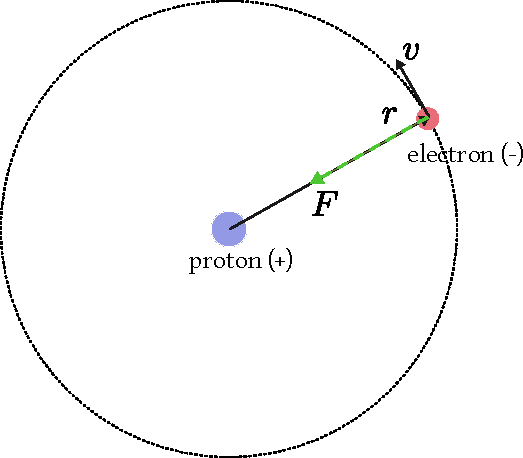
\includegraphics[scale=0.6]{hydrogenAtom}
	\caption{Planetary model of hydrogen atom.}
	\label{fig:hydrogenAtom}
\end{figure}

The circular motion of the electron around the nucleus is
mathematically similar to the problem of a planet circling a
star. Using the second law of Newton and the expression for the
Coulomb's force, we can write
\[
\frac{m_ev^2}{r} = k\frac{q_e^2}{r^2}\,,
\]
where
\[
k = \frac{1}{4\pi\varepsilon_0}\,.
\]

Newtonian momentum is given by $p=mv$; from the motion equation
above, we find
\[
p^2 = k\frac{m_e q_e^2}{r}\,.
\]

\begin{figure}[htbp]
	\centering
	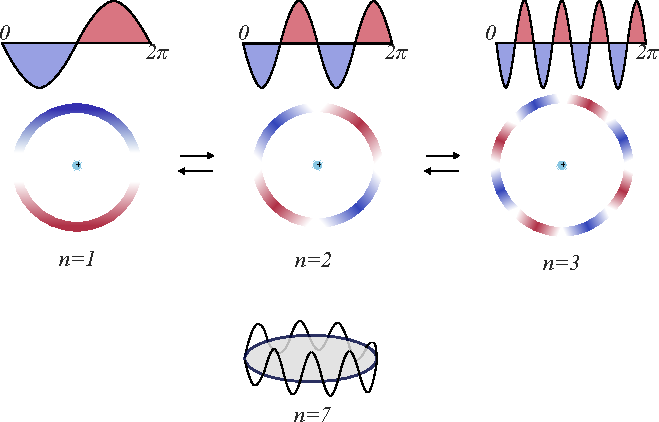
\includegraphics[scale=1.0]{hydrogenAtomOrbits}
	\caption{Orbits allowed by the semi-quantum model.}
	\label{fig:hydrogenAtomOrbits}
\end{figure}

Using de Broglie hypothesis about the relation between momentum and
wavelength
\[
p\lambda = h\,,
\]
and combining it with \emph{quantization hypothesis}:
\[
n\lambda = 2\pi r
\]
or, equivalently,
\[
pr = n\frac{h}{2\pi} = n\hbar\,
\]
we find possible solutions for the radius of the ``orbit'':
\[
r_n = \frac{\hbar^2 n^2}{km_e q_e^2}\qquad n = 1, 2, 3,\ldots
\]
The smallest value of the radius is
\[
a_0 = r_1 = \frac{4\pi\varepsilon_0 \hbar^2}{m_e q_e^2} = 0.523\,\r{A}\,.
\]
It is called \emph{Bohr radius}. Thus, the smallest diameter of
electron's orbit is about 1 \r{A}ngstrom.
\begin{exercise}
	Find the numbers for which the radius of electron ``orbit'' equals:
	1) 1 mm; 2) 1 cm; 3) 1 m.
\end{exercise}

How fast does the electron move around the nucleus? The velocity
of the electron is
\[
v = \sqrt{\frac{kq_e^2}{m_e r}}\,.
\]
Substituting $r_n = a_0 n^2$ we get
\[
v_n = \frac{1}{n}\sqrt{\frac{kq_e^2}{m_e a_0}} = \frac{v_1}{n}\,.
\]
The value of $v_1$ is
\[
v_1 = 2.19\times 10^6\,(m/s)
\]
Although this is a big number, it is much smaller than the speed of
light; we are therefore justified in using Newtonian mechanics and not
taking relativity into account.

\begin{tcolorbox}[colback=white!85!ocre, title=$\circledast\,$Fun Fact]
	The ``quantization'' of orbit radius can be found even for planets in
	solar system. If we denote the distance between the earth and the sun
	as $A$ (called \emph{astronomical unit}), then the distances to
	planets from the sun are given by the formula
	\[
	r_n = \frac{A}{10}(4+3\times 2^n)\,.
	\]
	This relation is known as \emph{Titius-Bode} law. It works remarkably
	well for all planets from Venus ($n=0$) to Uranus ($n=6$).
\end{tcolorbox}

How strong is the electron attracted to the nucleus? The Coulomb force
between the charges is
\[
F = \frac{kq_e^2}{r^2}\,.
\]
Substituting $r_n = a_0 n^2$ we get
\[
F_n = \frac{kq_e^2}{a_0^2 n^4} = \frac{F_1}{n^4}\,.
\]
The value of $F_1$ is
\[
F_1 = 8.24\times 10^{-8}\,(N)
\]
This is a tiny force on the human scale of forces.
\begin{tcolorbox}[colback=white!85!ocre, title=$\circledast\,$Fun Fact]
	Even a baby ant has enough force to tear a hydrogen atom apart with
	its bare hands!
\end{tcolorbox}
Although the force acting on the electron is small on a human scale,
the acceleration ($a=v^2/r$) it produces is very large (on the human
scale, compare to $g$). This is due to extreme lightness of the
electron:
\[
m_e = 9.1\times 10^{-31}\, (kg)\,.
\]

What is the total energy of the hydrogen atom? It can be found as
follows:
\[
E_n = \frac{m_ev_n^2}{2}-k\frac{q_e^2}{r_n} = -\frac{E_1}{n^2}\,,
\]
where
\[
E_1 = k\frac{q_e^2}{2m_e a_0}\,.
\]
The value of $E_1$ is
\[
E_1 = 2.18\times 10^{-18}\, (J)\,.
\]
In atomic world a special unit of energy is used. It is the energy of
electon accelerated by a voltage drop of 1 Volt:
\[
E_{ev} = 1\,(V)\times q_e = 1.6\times 10^{-19}\, (J)\,.
\]
Using this atomic unit, the hydrogen atom has energy
\[
E_1 = 13.6\, (eV)\,.
\]

\begin{exercise}
	What is the frequency of revolution of electron around the nucleus
	for an orbit number $n$?
\end{exercise}

\subsubsection{Atoms Can't Exist?}
The model described above leads to the conclusion that atoms must not
exist for long. According to the theory of classical electrodynamics,
a charge moving in a circle will emit electromagnetic
waves with the frequency of revolution. As the atom loses its energy,
the electron spirals ever closer to the nucleus. Taking classical
electrodynamics into account, the life-time of a hydrogen atoms should
be about nanosecond. This contradicts the observation of stability of
atoms.

Niels Bohr suggested that the ``orbits'' represent so called
\emph{stationary states}, where electrons can ``move'' without
radiating away electromagnetic waves. Radiation only happens when
electron \emph{transitions} between stationary levels, for example
between 2 and 4. The energy carried away by the light is related to
the frequency of the electromagnetic wave $\nu$ as follows:
\[
\Delta E = E_m - E_n = h\nu_{nm}\qquad m > n\,.
\]

%\begin{tcolorbox}[colback=white!85!ocre, title=Exercise]
\begin{exercise}
	How much energy is required to ``move'' electron from the``orbit''
	of 1 mm to 1 cm? From 1 cm to 1m?
\end{exercise}
%\end{tcolorbox}

\subsubsection{Line Spectra Explained}
Using the results obtained above, we can now describe the spectra of
light emitted or absorbed by hydrogen.

The stationary states are discrete, therefore there are discrete
energies of transition between a pair of levels. When atom absorbs
electromagnetic radiation, electron ``jumps up'' to higher energy
level and farther distance. In the reverse process, electron ``jumps
down'' from higher level to lower one, resulting in emission.

The wavelength of the radiation is
\[
\lambda = cT = \frac{c}{\nu} = \frac{ch}{E_m - E_n}\,.
\]
Plugging in the expression for the energy, we get
\begin{equation}
	\lambda = \frac{ch}{E_1}\frac{n^2m^2}{m^2-n^2} = 91.127(nm)\times\frac{n^2m^2}{m^2-n^2}\,.
	\label{eq:lambdaSeries}
\end{equation}

A special case of this formula was discovered in 1885 by a Swiss
mathematician Johan Balmer. Analyzing the visible lines in the spectra
of hydrogen, he found some regularity in the wavelengths. Balmer
expressed it as follows:
\[
\lambda = B\frac{m^2}{m^2-2^2}\,,
\]
where $m > 2$ and $B=364.51$ nm.
Looking at (\ref{eq:lambdaSeries}), we can see that it can be written
for $n=2$ as
\[
\lambda = 91.127(nm)\times \frac{4m^2}{m^2-2^2} = 364.51(nm)\times \frac{m^2}{m^2-2^2}\,.
\]

%\begin{tcolorbox}[colback=white!85!ocre, title=Exercise]
\begin{exercise}
	According to the the formula  (\ref{eq:lambdaSeries}), how many
	hydrogen lines will be in the visible part of the spectrum (from
	400nm to 700nm)?
\end{exercise}
%\end{tcolorbox}

\begin{mybio}{Three Body Problem}
	The problem of hydrogen atom involves \emph{three} physical entities
	interacting with each other: Proton, electron, and electromagnetic
	field. Electron does not interact directly with the proton, it does
	so via the electric field of the nucleus. This is important to keep
	in mind, especially if we want to understand the phenomenon of
	\emph{spontaneous emission}.
\end{mybio}
\subsubsection{Spontaneous Emission and Cavity QED}
According to Schrodinger equation, an hydrogen atom with electron in any
statioary state $\qs{\Psi_n}$ with energy $E_n$ will remain in this
state \emph{forever}. In reality, every atom will randomly transition
into a state with lower energy, all the way to the lowest energy
state, emitting radiation as the result. This is called \emph{spontaneous
	emission}.

To describe spontaneous emission, one must account for the fact that
atom is not truly isolated and electron and proton are not the only
quantum systems in picture. There is an electromagnetic field with its
many modes-oscillators.

Interaction of atom-like quantum systems (qubits, quantum dots, atoms)
with quantum states of electromagnetic field is the focus of an exctiting
area of research called \emph{Cavity Quantum Electrodynamics} or \emph{cavity QED}.
\begin{figure}[htbp]
	\centering
	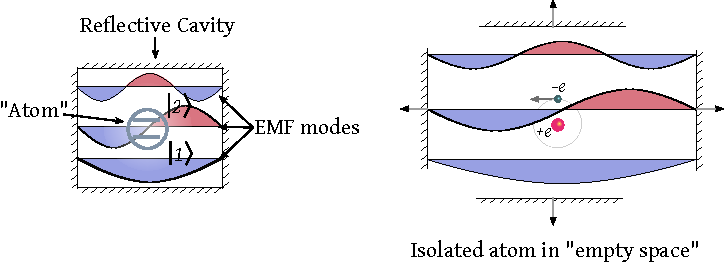
\includegraphics[scale=1.0]{cavityQED}
	\caption{Atom in ``empty space'' is a quantum system in a very large
		cavity, coupled to the modes-oscillators of electromagnetic field.}
	\label{fig:cavityQED}
\end{figure}

\subsection{Franck-Hertz Experiment}
The energy required for atoms to transition between different states may come not only from electromagnetic radiation ("photons"), but from kinetic energy of other particles bumping into atoms. Such a phenomenon was studied by James Franck and Gustav Hertz in 1914 using collisions of electrons with mercury atoms enclosed in a special vacuum tube. They showed that whenever electrons had a certain kinetic energy -- specific to mercury atoms -- they transfered this energy very efficiently (\emph{resonantly}) to mercury atoms. When the energies of electrons and mercury atoms were not matched, electrons scattered from the atoms \emph{elastically} -- without the loss of their kinetic energy.  The work of Franck and Hertz was recognized with 1925 Nobel Prize in Physics.

\subsubsection*{Idea}
The idea of Franck-Hertz experiment is illustrated in figure \ref{fig:franckHertzExperiment}. Its central part consists of a closed vacuum tube with mercury gas and several electric elements used as the source and sink of electrons.
\begin{figure}[htbp]
	\centering
	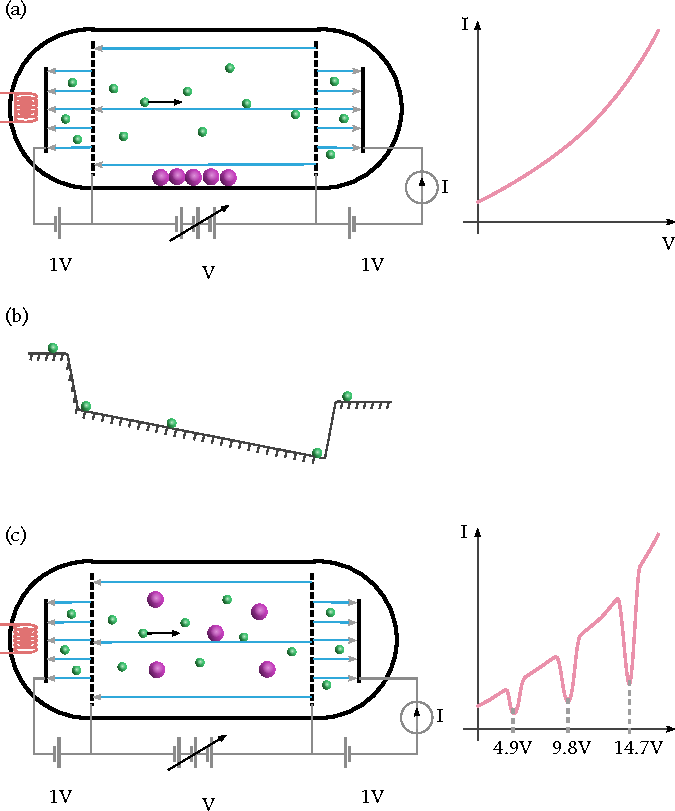
\includegraphics[scale=1.0]{franckHertzExperiment}
	\caption{(a) A vacuum tube is used to study the flow of electrons between two metal electrods under various conditions.; (b); (c).}
	\label{fig:franckHertzExperiment}
\end{figure}


\subsubsection*{Numbers}
At room temperature mercury is a liquid metal which can be easily evaporated by heating it up to 200$^\circ$C. It is thus not hard to create \emph{mercury gas}. The gas is \emph{monoatomic} -- consisting of single $Hg$ atoms, unlike molecular gases such as hydrogen $H_2$, oxigen $O_2$, or nitrogen $N_2$.

Each mercury atom contains 80 protons and 120 neutrons and is significantly heavier than an electron: $M_{Hg}\approx 4\times 10^5\,m_e$.  Consequently, an electron colliding with a mercury atom won't be able to impart any appreciable recoil speed or transfer energy to the latter. 
\begin{exercise}
	Show that for the head-on collision the speed of an initially stationary mercury atom after the collision becomes $v=2v_0\frac{m_e}{M_{Hg}}$.
\end{exercise}

\subsection{Stoke's Rule}
Stoke's rule.

\section{Rydberg Atoms}
When an atom has outer electron(s) excited into states with high excitation number  $n$, it is called a \emph{Rydberg atom}(CHECK!). Such atoms are of great importance for experiments of quantum physics.

\section{Quantum Dots}
Quantum dots can be viewed as \emph{artificial atoms} -- human-made physical structures designed to confine electrons in tiny volumes.
\[
\ketbra{\alpha}{\beta}
\]
\[
E_n = -\frac{E_i}{n^2}\,.
\]

\section{Spontaneous Emission}
\[
\ketbra{\alpha}{\beta}
\]
\[
E_n = -\frac{E_i}{n^2}\,.
\]

\section{Stimulated Emission}
\[
\ketbra{\alpha}{\beta}
\]
\[
E_n = -\frac{E_i}{n^2}\,.
\]

\section{Lasers}
\[
\ketbra{\alpha}{\beta}
\]
\[
E_n = -\frac{E_i}{n^2}\,.
\]



\section{Photoeffect}
\[
\ketbra{\alpha}{\beta}
\]
\[
E_n = -\frac{E_i}{n^2}\,.
\]

\section{Black Body Radiation}
\[
\rho_\nu = \frac{2h\nu^3}{c^2}\frac{1}{e^{h\nu/kT}-1}\,.
\]
\[
E_n = -\frac{E_i}{n^2}\,.
\]

\section{Conductors}
\[
\ketbra{\alpha}{\beta}
\]
\[
E_n = -\frac{E_i}{n^2}\,.
\]

\subsection{Heat Capacity}
Einstein's model.

\section{Entanglement}
\[
\ketbra{\alpha}{\beta}
\]
\[
E_n = -\frac{E_i}{n^2}\,.
\]

\subsubsection*{$\delta$-Notation}\index{Notation!delta}
When a quantity $x$ changes by a tiny amount, we will denote the
change using small Greek letter $\delta$ (delta) as follows:
\[
\colorboxed{red}{\delta x\textrm{ - tiny change of } x.}
\]
A convenient way to write all components of a second rank tensor is to
use table-like structure called \emph{matrix}\index{Matrix}:
\[
F^{\mu\nu}=
\begin{pmatrix}
  F^{00} & F^{01} & F^{02} & F^{03}\\
  F^{10} & F^{11} & F^{12} & F^{13}\\
  F^{20} & F^{21} & F^{22} & F^{23}\\
  F^{30} & F^{31} & F^{32} & F^{33}
\end{pmatrix}\,.
\]
In the matrix, the first index $\mu$ of $F^{\mu\nu}$ corresponds to
the row, while the second index $\nu$ corresponds to the column. Both
rows and columns are enumerated from $0$ to $3$.

Using matrix form, we can write the electromagnetic tensor in terms
of the electric and magnetic fields:
\[
F^{\mu\nu}=
\begin{pmatrix}
  0 & -\mathcal{E}^1 & -\mathcal{E}^2 & -\mathcal{E}^3\\
  \mathcal{E}^1 & 0 & -\mathcal{B}^3 & \mathcal{B}^2\\
  \mathcal{E}^2 & \mathcal{B}^3 & 0 & -\mathcal{B}^1\\
  \mathcal{E}^3 & -\mathcal{B}^2 & \mathcal{B}^1 & 0
\end{pmatrix}\,.
\]


\section*{Chapter Highlights}
{\setstretch{1.5}\chhc
  \it
\begin{itemize}
\item Tensors find application in various areas of science and math.
\item Geometrical properties of surfaces and spaces can be described
  using metric tensor.
\item Physical properties of solids are often anisotropic -- depend on
  the direction of applied ``force''. Such properties are best
  described by various tensors: stress tensor, mobility tensor,
  piezoelectric tensor, and others.
\item At the fundamental level electric and magnetic fields are united
  in a single physical object -- electromagnetic field. Electromagnetic
  field is described by an antisymmetric tensor of the second rank.
\end{itemize}

}
